
\documentclass[10pt,a4paper]{article}
\usepackage[T1]{fontenc}
\usepackage{tikz}
\usepackage[margin=1cm]{geometry}
\begin{document}

\section*{Final Binary Search Tree}
This document presents the final binary search tree (BST) generated through a sequence of node insertions. The tree is constructed by adding nodes in accordance with BST properties, where each node has a left child with a smaller value and a right child with a larger value.

\subsection*{Tree Construction Algorithm}
The binary search tree was constructed using the following algorithm:
\begin{enumerate}
    \item \textbf{Initialization:} Start with an empty tree.
    \item \textbf{Insert Root Node:} The first node inserted becomes the root of the tree.
    \item \textbf{Insert Subsequent Nodes:} For each new node:
    \begin{itemize}
        \item Compare the value of the new node with the current node.
        \item If the new node's value is less, move to the left child; if greater, move to the right child.
        \item Repeat the comparison until finding an appropriate empty position.
    \end{itemize}
    \item \textbf{Recursive Insertion:} Continue recursively inserting nodes to maintain the BST properties.
\end{enumerate}

\subsection*{Final Tree Visualization}
The final binary search tree, after all nodes have been inserted, is visualized below:

\begin{center}
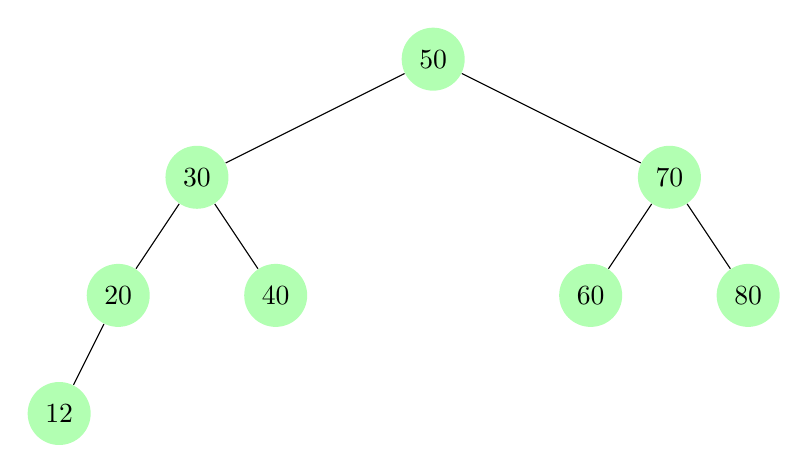
\begin{tikzpicture}[level distance=15mm, sibling distance=20mm]
    \tikzstyle{every node}=[circle,inner sep=1pt, minimum size=8mm]
    \tikzstyle{level 1}=[sibling distance=60mm]
    \tikzstyle{level 2}=[sibling distance=20mm]
    \tikzstyle{level 3}=[sibling distance=15mm]
    \tikzstyle{level 4}=[sibling distance=10mm]

% The following code generates the final binary search tree (BST) after all insertions.

    \node [fill=green!30] {50} child {node [fill=green!30] {30} child {node [fill=green!30] {20} child {node [fill=green!30] {12} } child[fill=none] {edge from parent[draw=none]}} child {node [fill=green!30] {40} }} child {node [fill=green!30] {70} child {node [fill=green!30] {60} } child {node [fill=green!30] {80} }};

\end{tikzpicture}
\end{center}

\end{document}
